\documentclass[12pt]{article}
\usepackage[margin=1in]{geometry} 
\usepackage{graphicx}
\usepackage{amsmath,amsthm,amssymb}
\usepackage{hyperref}
\usepackage{tikz}

\title{
    \textbf{Theory Assignment 5} \\ 
    \textbf{CS5280} \\
}

\author{
    \textbf{Darpan Gaur} \\
    \textbf{CO21BTECH11004}
}


\date{}

\begin{document}
\maketitle

\hrulefill

\section*{Problem 6.3}
\subsection*{1st Schedule}
Deposit(c) for both transactions $t_1$ and $t_2$ are isolated. 
As shown in figure \ref{fig:1}, we can isolate Withdraw(a) and Withdraw(b) by pushing r(q) of Withdraw(a) to right of w(t) of Withdraw(b). 
Now as all operations at level 1 are isolated we can prune operations at level 0 in the tree.
\begin{figure}[h]
    \centering
    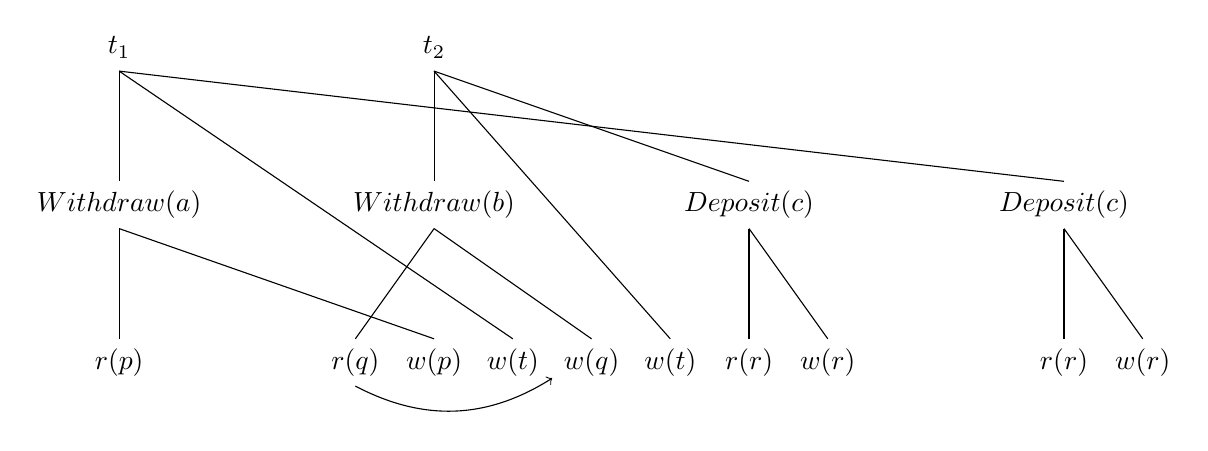
\begin{tikzpicture}
        \node at (0, 0) {\(t_1\)};
        \node at (4, 0) {\(t_2\)};

        \node at (0, -2) {\(Withdraw(a)\)};
        \node at (4, -2) {\(Withdraw(b)\)};
        \node at (8, -2) {\(Deposit(c)\)};
        \node at (12, -2) {\(Deposit(c)\)};

        \node at (0, -4) {\(r(p)\)};
        \node at (3, -4) {\(r(q)\)};
        \node at (4, -4) {\(w(p)\)};
        \node at (5, -4) {\(w(t)\)};
        \node at (6, -4) {\(w(q)\)};
        \node at (7, -4) {\(w(t)\)};

        \node at (8, -4) {\(r(r)\)};
        \node at (9, -4) {\(w(r)\)};

        \node at (12, -4) {\(r(r)\)};
        \node at (13, -4) {\(w(r)\)};

        \draw[-] (0, -0.3) -- (0, -1.7);
        \draw[-] (0, -0.3) -- (5, -3.7);
        \draw[-] (0, -0.3) -- (12, -1.7);

        \draw[-] (4, -0.3) -- (4, -1.7);
        \draw[-] (4, -0.3) -- (7, -3.7);
        \draw[-] (4, -0.3) -- (8, -1.7);

        \draw[-] (0, -2.3) -- (0, -3.7);
        \draw[-] (0, -2.3) -- (4, -3.7);

        \draw[-] (4, -2.3) -- (3, -3.7);
        \draw[-] (4, -2.3) -- (6, -3.7);

        \draw[-] (8, -2.3) -- (8, -3.7);
        \draw[-] (8, -2.3) -- (9, -3.7);

        \draw[-] (12, -2.3) -- (12, -3.7);
        \draw[-] (12, -2.3) -- (13, -3.7);

        % make a curve line between (0, -1.7) and (4, -1.7), having one end as arrow
        \draw[->] (3, -4.3) to [bend right=30] (5.5, -4.2);
    \end{tikzpicture}
    \caption{Commute of r(q) in 1st schedule}
    \label{fig:1}
\end{figure}\\
As shown in figure \ref{fig:2}, we can isolate $t_1$ and $t_2$ by pushing Deposit(c) of $t_1$ to the left of Withdraw(b) of $t_2$.
Now as all operations at level 1 are isolated we can prune operations at level 0 in the tree. As we are only left with root nodes, hence 1st schedult is tree reducible.
The serialization order is $t_1$ then $t_2$.
\begin{figure}[h]
    \centering
    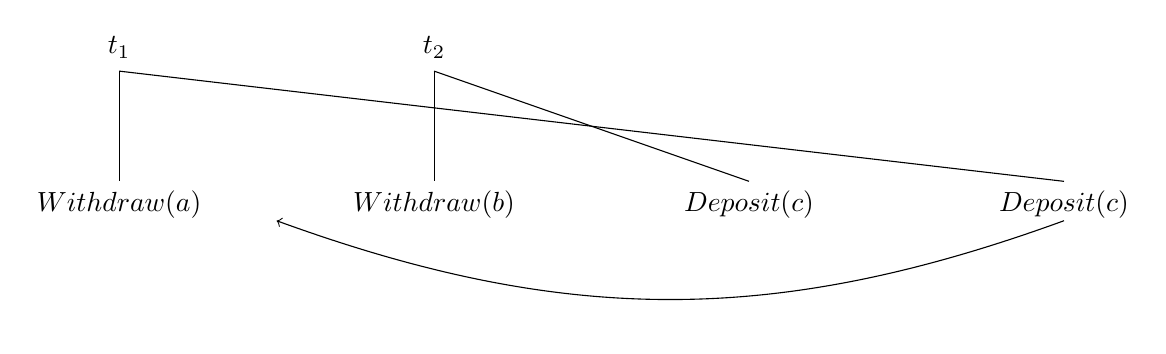
\begin{tikzpicture}
        \node at (0, 0) {\(t_1\)};
        \node at (4, 0) {\(t_2\)};

        \node at (0, -2) {\(Withdraw(a)\)};
        \node at (4, -2) {\(Withdraw(b)\)};
        \node at (8, -2) {\(Deposit(c)\)};
        \node at (12, -2) {\(Deposit(c)\)};
        
        \draw[-] (0, -0.3) -- (0, -1.7);
        \draw[-] (0, -0.3) -- (12, -1.7);

        \draw[-] (4, -0.3) -- (4, -1.7);
        \draw[-] (4, -0.3) -- (8, -1.7);

        \draw[->] (12, -2.2) to [bend left=20] (2, -2.2);
    \end{tikzpicture}
    \caption{Commute of Deposit(c) in 1st schedule}
    \label{fig:2}
\end{figure}\\

\subsection*{2nd Schedule}
As shown in figure \ref{fig:3}, we can isolate Withdraw(a) and Withdraw(b) by pushing r(q) of Withdraw(a) to right of w(t) of Withdraw(b). 
\begin{figure}[h]
    \centering
    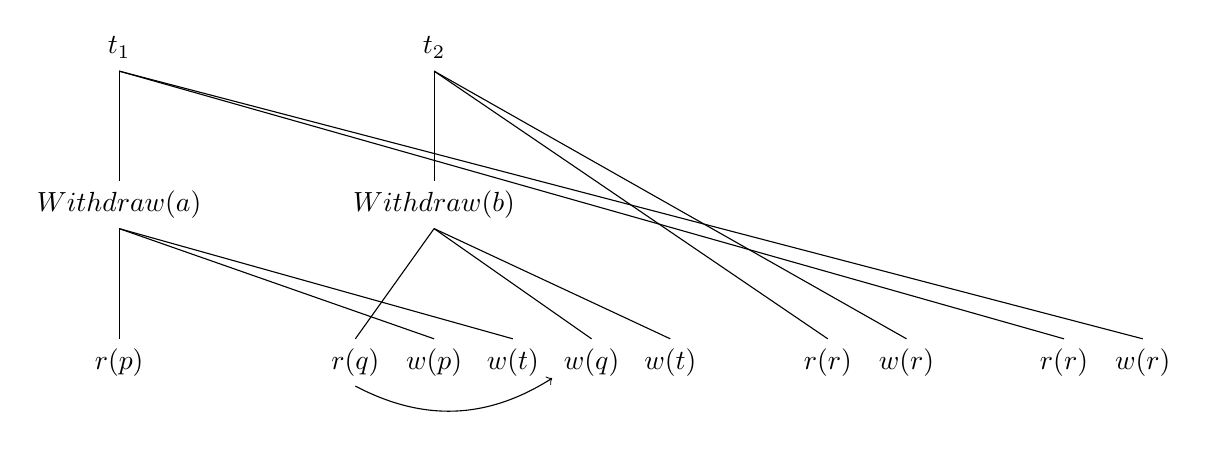
\begin{tikzpicture}
        \node at (0, 0) {\(t_1\)};
        \node at (4, 0) {\(t_2\)};

        \node at (0, -2) {\(Withdraw(a)\)};
        \node at (4, -2) {\(Withdraw(b)\)};
        
        \node at (0, -4) {\(r(p)\)};
        \node at (3, -4) {\(r(q)\)};
        \node at (4, -4) {\(w(p)\)};
        \node at (5, -4) {\(w(t)\)};
        \node at (6, -4) {\(w(q)\)};
        \node at (7, -4) {\(w(t)\)};

        \node at (9, -4) {\(r(r)\)};
        \node at (10, -4) {\(w(r)\)};

        \node at (12, -4) {\(r(r)\)};
        \node at (13, -4) {\(w(r)\)};

        \draw[-] (0, -0.3) -- (0, -1.7);
        \draw[-] (0, -0.3) -- (12, -3.7);
        \draw[-] (0, -0.3) -- (13, -3.7);

        \draw[-] (4, -0.3) -- (4, -1.7);
        \draw[-] (4, -0.3) -- (9, -3.7);
        \draw[-] (4, -0.3) -- (10, -3.7);

        \draw[-] (0, -2.3) -- (0, -3.7);
        \draw[-] (0, -2.3) -- (4, -3.7);
        \draw[-] (0, -2.3) -- (5, -3.7);

        \draw[-] (4, -2.3) -- (3, -3.7);
        \draw[-] (4, -2.3) -- (6, -3.7);
        \draw[-] (4, -2.3) -- (7, -3.7);

        \draw[->] (3, -4.3) to [bend right=30] (5.5, -4.2);
    \end{tikzpicture}
    \caption{Commute of r(q) in 2nd schedule}
    \label{fig:3}
\end{figure} \\
As shown in figure \ref{fig:4}, we can commute Withdraw(a) and Withdraw(b) as they are operating on different data-items and are isolates. 
Underlying operations of Withdraw(a) are not conflicting with $t_2$ r(r) and w(r), we can commute them. Shift Withdraw(a) after $t_2$. 
Now as all operations at root are isolated, hence tree is reducible. Execution order is $t_2$ then $t_1$.
\begin{figure}[h]
    \centering
    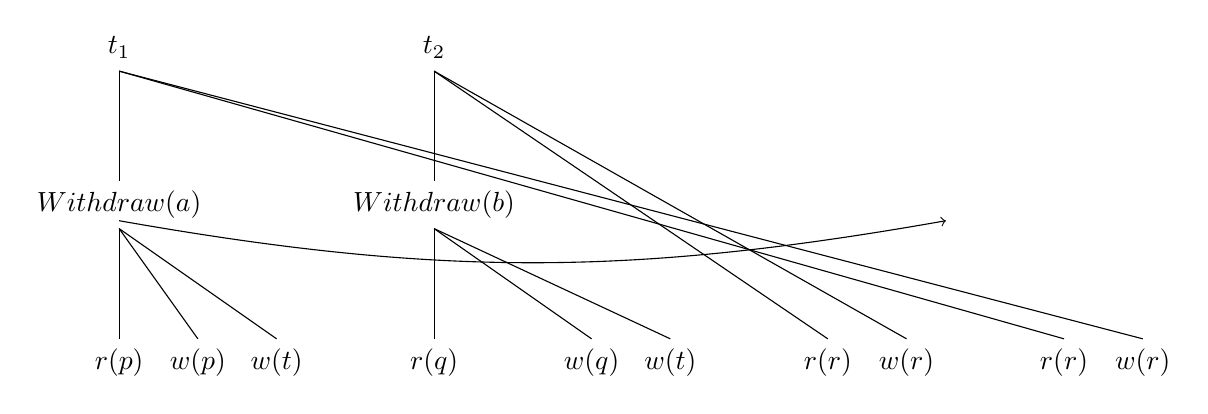
\begin{tikzpicture}
        \node at (0, 0) {\(t_1\)};
        \node at (4, 0) {\(t_2\)};

        \node at (0, -2) {\(Withdraw(a)\)};
        \node at (4, -2) {\(Withdraw(b)\)};
        
        \node at (0, -4) {\(r(p)\)};
        \node at (4, -4) {\(r(q)\)};
        \node at (1, -4) {\(w(p)\)};
        \node at (2, -4) {\(w(t)\)};
        \node at (6, -4) {\(w(q)\)};
        \node at (7, -4) {\(w(t)\)};

        \node at (9, -4) {\(r(r)\)};
        \node at (10, -4) {\(w(r)\)};

        \node at (12, -4) {\(r(r)\)};
        \node at (13, -4) {\(w(r)\)};

        \draw[-] (0, -0.3) -- (0, -1.7);
        \draw[-] (0, -0.3) -- (12, -3.7);
        \draw[-] (0, -0.3) -- (13, -3.7);

        \draw[-] (4, -0.3) -- (4, -1.7);
        \draw[-] (4, -0.3) -- (9, -3.7);
        \draw[-] (4, -0.3) -- (10, -3.7);

        \draw[-] (0, -2.3) -- (0, -3.7);
        \draw[-] (0, -2.3) -- (1, -3.7);
        \draw[-] (0, -2.3) -- (2, -3.7);

        \draw[-] (4, -2.3) -- (4, -3.7);
        \draw[-] (4, -2.3) -- (6, -3.7);
        \draw[-] (4, -2.3) -- (7, -3.7);

        \draw[->] (0, -2.2) to [bend right=10] (10.5, -2.2);
    \end{tikzpicture}
    \caption{Commute of Withdraw(a) in 2nd schedule}
    \label{fig:4}
\end{figure}

\clearpage

\section*{Problem 6.6}
Table \ref{tab:ct} shows the commutativity of return values of operations for the counter object.
\begin{table}[h!]
    \centering
    \renewcommand{\arraystretch}{1.3}
    \setlength{\tabcolsep}{10pt}
    \begin{tabular}{|c|c|c|c|c|c|c|}
    \hline
     & \textit{Inc} $\uparrow$ \textit{OK} & \textit{Inc} $\uparrow$ \textit{No} & \textit{Dec} $\uparrow$ \textit{OK} & \textit{Dec} $\uparrow$ \textit{No} & \textit{GV} $\uparrow$ \textit{x} \\
    \hline
    \textit{Inc} $\uparrow$ \textit{OK} & $+$ & $-$ & $-$ & $+$ & $-$ \\
    \textit{Inc} $\uparrow$ \textit{No} & $+$ & $+$ & $-$ & $+$ & $+$ \\
    \textit{Dec} $\uparrow$ \textit{OK} & $-$ & $+$ & $+$ & $-$ & $-$ \\
    \textit{Dec} $\uparrow$ \textit{No} & $-$ & $+$ & $+$ & $+$ & $+$ \\
    \textit{GV} $\uparrow$ \textit{x} & $-$ & $+$ & $-$ & $+$ & $+$ \\
    \hline
    \end{tabular}
    \caption{Return value commutativity table}
    \label{tab:ct}
\end{table}\\
Following improvements of concurrency can be done:
\begin{itemize}
    \item $dec(x, \Delta_1) \uparrow No$ and $inc(x, \Delta_2) \uparrow OK$: If $x + \Delta_2 - \Delta_1 \leq lower\_bound$, then they are commutable.
    \item $inc(x, \Delta_1) \uparrow No$ and $dec(x, \Delta_2) \uparrow OK$: If $x + \Delta_1 - \Delta_2 \geq upper\_bound$, then they are commutable.
    \item $dec(x, \Delta_1) \uparrow OK$ and $inc(x, \Delta_2) \uparrow OK$: If $x + \Delta_2 \leq upper\_bound$ then they are commutable.
    \item $inc(x, \Delta_1) \uparrow OK$ and $dec(x, \Delta_2) \uparrow OK$: If $x - \Delta_2 \geq lower\_bound$ then they are commutable.
    \item $dec(x, \Delta_1) \uparrow OK$ and $dec(x, \Delta_2) \uparrow No$: If $x - \Delta_2 \leq lower\_bound$ then they are commutable.
    \item $inc(x, \Delta_1) \uparrow OK$ and $inc(x, \Delta_2) \uparrow No$: If $x + \Delta_2 \geq upper\_bound$ then they are commutable.
\end{itemize}

\section*{Problem 7.1}
Under layered sysytem with layered 2PL, deadlock can occur in two ways:
\begin{itemize}
    \item Local deadlock: Transactions are wating for each to release the locks due to operations on same layer.
    \item Global deadlock: Transactions are waiting for each to release the locks due to operations on different layers.
\end{itemize}
\subsection*{Local Deadlocks}
In figure \ref{fig:d1}, $t_1$ acquires lock on Withdraw(a), then $t_2$ acquires lock on Withdraw(b) and $t_3$ acquires lock on Withdraw(c).
Now $t_1$ is waiting for lock on Deposit(b) which is held by $t_2$, $t_2$ is waiting for lock on Deposit(c) which is held by $t_3$ and $t_3$ is waiting for lock on Deposit(a) which is held by $t_1$.
This is a deadlock as all transactions are waiting for each other to release the locks. As all are on same layer, hence it is a deadlock within same layer.
Here, transactions are blocked at level $L_i$ and if it dosen't hold locks at lower levels, it can't be blocked by any other object below level $L_i$.
\begin{figure}[h]
    \centering
    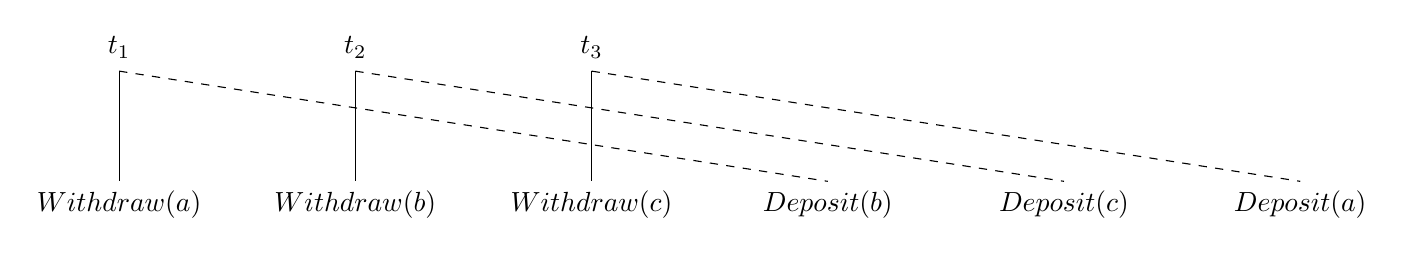
\begin{tikzpicture}
        \node at (0, 0) {\(t_1\)};
        \node at (3, 0) {\(t_2\)};
        \node at (6, 0) {\(t_3\)};
        
        \node at (0, -2) {\(Withdraw(a)\)};
        \node at (3, -2) {\(Withdraw(b)\)};
        \node at (6, -2) {\(Withdraw(c)\)};

        \node at (9, -2) {\(Deposit(b)\)};
        \node at (12, -2) {\(Deposit(c)\)};
        \node at (15, -2) {\(Deposit(a)\)};

        \draw[-] (0, -0.3) -- (0, -1.7);
        \draw[dashed] (0, -0.3) -- (9, -1.7);
        \draw[-] (3, -0.3) -- (3, -1.7);
        \draw[dashed] (3, -0.3) -- (12, -1.7);
        \draw[-] (6, -0.3) -- (6, -1.7);
        \draw[dashed] (6, -0.3) -- (15, -1.7);
    \end{tikzpicture}
    \caption{Local deadlock: within same layer }
    \label{fig:d1}
\end{figure}

\subsection*{Global Deadlocks}
In figure \ref{fig:d2}, $t_1$ acquires lock on r(a) and $t_2$ executes Withdraw(x) and acquires lock on r(a). Now $t_2$ is waiting for lock on w(a) as it conflicts with r(a) of $t_1$.
$t_1$ is waiting for lock on Deposit(x) which is conflicting with Withdraw(x) of $t_2$.
This is a deadlock as both transactions are waiting for each other to release the locks. As they are on different layers, hence it is a global deadlock.
\begin{figure}[h]
    \centering
    \begin{tikzpicture}
        \node at (0, 0) {\(t_1\)};
        \node at (2, 0) {\(t_2\)};

        \node at (0, -4) {\(r(a)\)};
        \node at (2, -2) {\(Withdraw(x)\)};
        \node at (2, -4) {\(r(a)\)};
        \node at (3, -4) {\(w(a)\)};

        \node at (5, -2) {\(Deposit(x)\)};

        \draw[-] (0, -0.3) -- (0, -3.7);
        \draw[-] (2, -0.3) -- (2, -1.7);
        \draw[dashed] (0, -0.3) -- (5, -1.7);
        \draw[-] (2, -2.2) -- (2, -3.7);
        \draw[dashed] (2, -2.2) -- (3, -3.7);
    \end{tikzpicture}
    \caption{Global deadlock: cross layer}
    \label{fig:d2}
\end{figure}

\end{document}


